\documentclass[12pt]{article}
\usepackage[utf8]{inputenc}
\usepackage{amsmath}
\usepackage{amsfonts}
\usepackage{amssymb}
\usepackage{graphicx}
\graphicspath{ {./img/} }
\usepackage{hyperref}
\usepackage{array}
\usepackage{multirow}
\usepackage{longtable}
\usepackage{enumitem}
\usepackage{fancyvrb}
\usepackage[a4paper, total={6in, 8in}]{geometry}
\usepackage[table,xcdraw]{xcolor}
\usepackage{makecell}

\usepackage{titlesec}

\setcounter{secnumdepth}{4}

\newcounter{mycounter} 
\newcommand\showmycounter{\stepcounter{mycounter}\themycounter}

\titleformat{\paragraph}
{\normalfont\normalsize\bfseries}{\theparagraph}{1em}{}
\titlespacing*{\paragraph}
{0pt}{3.25ex plus 1ex minus .2ex}{1.5ex plus .2ex}

\author{Natale Guadagno, Paolo Patrone}
\title{Test Report - TecStore}
\renewcommand{\contentsname}{Contenuti}

\usepackage{hyperref}
\hypersetup{
    colorlinks,
        citecolor=blue,
    filecolor=blue,
    linkcolor=blue,
    urlcolor=blue,
    linktocpage
}

\begin{document}

\maketitle
\newpage
\tableofcontents
\newpage
\newgeometry{a4paper,textwidth=345pt,textheight=598pt}
\section*{Partecipanti}
\begin{center}
\begin{tabular} {|c|c|}
\hline
\textbf{Nome} & \textbf{Matricola} \\
\hline
Guadagno Natale & 0512106546 \\
Patrone Paolo & 0512106153 \\
\hline
\end{tabular}
\end{center}


\section*{Revision History}
\begin{center}
\begin{tabular} {|c|c|c|}
\hline
\textbf{Data} & \textbf{Versione} & \textbf{Descrizione} \\
21/2/2022 & 0.1 & Prima stesura \\
\hline

\hline
\end{tabular}
\end{center}

\newpage

\section{Metodologie di testing}
Si è scelto di dividere il testing in due fasi principali:
\subsection{JUnit}
Una volta raggiunta un'implementazione completa, ci si è adoperati per scrivere dei test JUnit che mettessero alla prova le funzioni principali dei model, in maniera tale da rilevare eventuali errori nel codice o nell'esecuzione di particolari operazioni. \\
Si sono usati gli strumenti messi a disposizione da Eclipse IDE for Java EE per scrivere ed eseguire i test. \\ \\

Da questo testing sono emerse svariate problematiche legate alla logica interna di alcune funzioni, dei Bean e alla struttura del database, che sono state prontamente risolte. \\ \\
Poiché i test sono eseguiti sequenzialmente e un reset totale del database tra un test e l'altro rallenterebbe enormemente la fase di esecuzione dei test, è stato necessario rinominare alcuni dei test aggiungendo dei suffissi affinché, rispettando l'ordine alfabetico, l'ordine delle operazioni sia sempre possibile: ad esempio, se si tentasse di rimuovere un articolo o di modificarne le informazioni prima che venga inserito, ci sarebbero ovviamente degli errori.


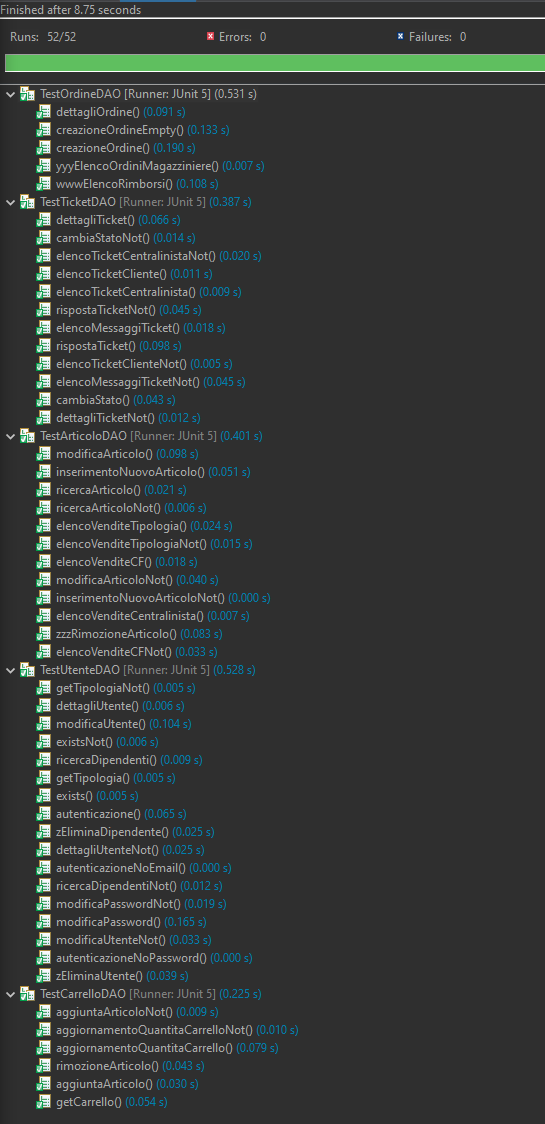
\includegraphics[width=\textwidth]{JUnit}

\subsection{Selenium}
In seguito al testing JUnit e alle dovute modifiche al sistema, accertatisi della funzionalità quasi certa dei DAO si è usata la libreria Selenium per testare le servlet e le loro risposte. \\
Si è usato lo strumento Selenium IDE, un'estensione per browser che ha permesso di velocizzare enormemente la fase di scrittura dei test, riducendo al minimo la necessità di scrivere ulteriore codice. \\ \\

Anche in questo caso sono emerse svariate criticità nell'esecuzione delle operazioni, che sono state risolte anche tramite la stesura dei test, che hanno velocizzato la fase di verifica del nuovo codice. \\ \\
Come per i test JUnit, la sequenzialità delle operazioni è stato un fattore di cui si è tenuto conto nella stesura dei test, affinché, ammesso di partire da un database in cui esistono solo dei dati predefiniti, i test non falliscano a causa di dati estranei o imprevisti.



\end{document}
